%% LyX 2.0.5.1 created this file.  For more info, see http://www.lyx.org/.
%% Do not edit unless you really know what you are doing.
\documentclass[usenatbib]{article}
\usepackage[latin9]{inputenc}
\usepackage[a4paper]{geometry}
\geometry{verbose}
\usepackage{color}
\usepackage{float}
\usepackage{graphicx}

\makeatletter

%%%%%%%%%%%%%%%%%%%%%%%%%%%%%% LyX specific LaTeX commands.
%% Because html converters don't know tabularnewline
\providecommand{\tabularnewline}{\\}
%% A simple dot to overcome graphicx limitations
\newcommand{\lyxdot}{.}


%%%%%%%%%%%%%%%%%%%%%%%%%%%%%% Textclass specific LaTeX commands.
\usepackage{jcappub}

%%%%%%%%%%%%%%%%%%%%%%%%%%%%%% User specified LaTeX commands.






%%%%%%%%%%%%%%%%%%%%%%%%%%%%%% LyX specific LaTeX commands.
%% A simple dot to overcome graphicx limitations
%Make my life significantly easier
\global\long\def\bd{{\bm{\delta}}}

\usepackage{astrobib_mnras2e}

\bibliographystyle{JHEP}

\makeatother

\begin{document}

\title{Generating Mock Catalogs for the Baryon Oscillation Spectroscopic
Survey: An Approximate N-Body approach}


\author{Tomomi Sunayama\textsuperscript{a}, Nikhil Padmanabhan\textsuperscript{a},
Katrin Heitmann\textsuperscript{b}, Salman Habib\textsuperscript{b},
Steve Rangel\textsuperscript{b,c}}


\abstract{Precision measurements of the large scale structure of the Universe
require large numbers of high fidelity mock catalogs to accurately
assess, and account for, the presence of systematic effects. We introduce
and test a scheme for generating mock catalogs rapidly using suitably
derated N-body simulations. Our aim is to reproduce the large scale
structure and the gross properties of dark matter halos with high
accuracy, while sacrificing the details of the halo's internal structure.
By adjusting global and local time-steps in an N-body code, we demonstrate that we 
recover halo masses to better than $2\%$ and the power spectrum (both in 
real and redshift space, for $k=1h{\rm Mpc^{-1}}$)
to better than $1\%$, while requiring a factor of 4 less CPU time.
We also calibrate the redshift
spacing of outputs required to generate simulated light cones. We
find that outputs separated by $\Delta z=0.05$ allow us to interpolate
particle positions and velocities to reproduce
the real and redshift space power spectra to better than $1\%$ (out
to $k=1h{\rm Mpc^{-1}}$). 
We apply these ideas to generate a suite of simulations spanning a range
of cosmologies, motivated by the Baryon Oscillation Spectroscopic Survey (BOSS) but
broadly applicable to future large scale structure surveys including eBOSS and
DESI. As an initial demonstration of the utility of such simulations, we 
calibrate the shift in the BAO position as a function of galaxy bias with 
higher precision than has been possible before. This paper also serves to 
document these simulations, which we make publically available.
}


\affiliation{\textsuperscript{a}Yale University, New Haven, CT}


\affiliation{\textsuperscript{b }Argonne National Laboratory, Lemont, IL}


\affiliation{\textsuperscript{c }Northwestern University, Evanston, IL}


\emailAdd{tomomi.sunayama@yale.edu, nikhil.padmanabhan@yale.edu,heitmann@anl.gov,
habib@anl.gov,steverangel@u.northwestern.edu }


\keywords{cosmology; large-scale structure of Universe, cosmological parameters,
galaxies; halos, statistics}

\maketitle

\section{Introduction}

Large-volume spectroscopic surveys of the Universe \citep{2013arXiv1305.5422S,2000AJ....120.1579Y,2011MNRAS.415.2876B}
are revolutionizing our understanding of cosmology and structure
formation. Based on these successes, a new generation of surveys \citep{2013arXiv1308.0847L,2013arXiv1305.5422S,2011arXiv1110.3193L}
is being planned that will improve our constraints by an order of
magnitude (or more). This unprecedented improvement in statistical
precision places stringent demands on the theoretical modeling and
analysis techniques; simulations will play an essential in meeting
these requirements.

One of the challenges for simulations are the varied roles they play,
and the different requirements these impose on the simulations. At
one extreme, simulations are necessary for estimating the errors on the 
measurements.
This typically requires very large
volumes to simulate entire surveys thousands of times, but have lower
accuracy requirements. Motivated by these considerations, a number
of recent studies have investigated methods designed to produce mock
catalogs with reduced accuracy, but much higher throughput compared
to the full N-body simulations~\cite{2002ApJ...564....8M,2002MNRAS.331..587M,2008MNRAS.391..435F,
2013AN....334..691R,2013arXiv1312.2013C,2013JCAP...06..036T,2014MNRAS.437.2594W,
2013MNRAS.433.2389M,2001A&A...367...18H,2009ApJ...701..945S,2014MNRAS.439L..21K,2014arXiv1409.1124C}.
An open question still is the effect of changing the input cosmology
used to generate the covariance matrix on cosmological inferences,
and how best to implement such variations (but see \citep{Kalus2015} for 
recent work on this). More recently, the impact
of super-survey modes (modes outside the survey volume) on inferred
errors has been shown to be potentially larger than previously appreciated
\citep[eg.][]{2013PhRvD..87l3504T} and is an area
of active study.

At the other extreme, simulations are crucial for calibrating the
theoretical models used to fit the data. Examples here are quantifying
shifts in the baryon acoustic oscillation distance scale due to nonlinear
evolution and galaxy bias \citep{2008ApJ...686...13S,2008PhRvD..77b3533C,2008PhRvD..77d3525S,2009PhRvD..80f3508P,2010ApJ...720.1650S,2012PhRvD..85j3523S},
or templates used to fit the full shape of the galaxy correlation function.
For such applications, one ideally requires high fidelity simulations.
The volume requirements are significantly reduced from that for covariance
matrices, but still need to much larger than survey volumes to keep
systematic errors below statistical errors.

An intermediate application are the generation of mock catalogs that
capture the observational characteristics of surveys (eg. geometry,
selection effects). The importance of these cannot be underestimated,
since the effects of many observational systematics can only be quantitatively
estimated by simulating them. These issues will get progressively
more important for the next generations of surveys which will move
away from highly complete and pure samples that have mostly been used
for cosmological studies to date.

The simplest way to generate approximate density fields is to use
analytic approximations such as Lagrangian perturbation theory followed
by prescriptions to put in halos in a way that better matches results
from N-body simulations~\cite{2013MNRAS.428.1036M,2014arXiv1401.4171M},
or simply to run lower resolution N-body codes with a small number
of time-steps~\cite{2013JCAP...06..036T}, or a combination of the
two approaches~\cite{2014MNRAS.437.2594W}. These methods are successful
in capturing the large-scale density field but lose information at
small scales. Because of their speed, they can be used to produce
large numbers of simulations required to build sample covariance matrices,
at error levels ranging from $5-10\%$ (depending on the quantities
being predicted). It is difficult to estimate, however, what the loss
of accuracy implies for tests of systematic errors, which may need
to be modeled at the $< 1\%$ level.

The approach we take here is to reduce the small-scale accuracy of
a high-resolution N-body code by coarsening its temporal resolution.
For the code we consider here, the time-stepping consists of two components,
(i) a long time step for solving for evolution under the long-range
particle-mesh (PM) force, and (ii) a set of underlying sub-cycled
time steps for a short-range particle-particle interaction, computed
either via a tree-based algorithm, or by direct particle-particle
force evaluations. The idea is to reduce the number of both types
of time steps while preserving enough accuracy to correctly describe
the large scale distribution of galaxies, as modeled by a halo occupation
distribution (HOD) approach. Our first goal in this paper is, therefore,
to quantitatively understand the impact of the temporal resolution
on the halo density field and how best to accurately reproduce the
details of the halo density field on large scales, sacrificing small
scale structure information. This allows to generate a suite of large
volume simulations, spanning a range of cosmologies. This paper presents
the details of these simulations and outlines future applications.

This paper is organized as follows. Sec.~2 briefly describes the
Hardware/Hybrid Accelerated Cosmology Code (HACC) N-body framework
we use to generate our simulations, focusing on the flexibility in
the time-stepping that we exploit here. Sec.~3 presents a sequence
of convergence tests where we evaluate the effects of time-stepping
on the halo density field. Sec.~4 discusses interpolating between
saved time steps, necessary for constructing light-cone outputs. Sec.~5
presents two example applications of these simulations : generating
mock catalogs that match the BOSS galaxy sample, and calibrating
shifts in the baryon acoustic oscillation (BAO) scale. We conclude in Sec.~6
by outlining possible future directions.

Unless specified, all simulations and calculations in this paper assume a $\Lambda$CDM
cosmology with $\Omega_{m}=0.2648$, $\Omega_{\Lambda}=0.7352$, $\Omega_{b}h^{2}=0.02258$,
$n_{s}=0.963$, $\sigma_{8}=0.8$ and $h=0.71$.


\section{HACC}

All simulations in this paper were carried out using the HACC (Hardware/Hybrid
Accelerated Cosmology Code) framework. HACC provides an advanced,
architecture-agile, extreme-scale N-body capability targeted to cosmological
simulations. It is descended from an approach originally developed
for the heterogeneous architecture of Roadrunner \cite{1742-6596-180-1-012019,Pope:2010:AU:1845737.1845828},
the first computer to break the petaflop performance barrier.

HACC's flexible code architecture combines MPI with a variety of more
local programming models, (e.g., OpenCL, OpenMP) and is easily adaptable
to different platforms. HACC has demonstrated scaling on the entire
IBM BG/Q Sequoia system up to 1,572,864 cores with an equal number
of MPI ranks, attaining 13.94 PFlops at 69.2\% of peak and 90\% parallel
efficiency (for details, see \citep{2012arXiv1211.4864H}). Examples
of science results obtained using HACC include 64-billion particle
runs for baryon acoustic oscillations predictions for the BOSS Lyman-$\alpha$
forest \cite{2010ApJ...713..383W}, high-statistics predictions for
the halo profiles of massive clusters \cite{2013ApJ...766...32B},
and 0.5 and 1.1~trillion particle runs at high mass resolution. A
recent overview of the HACC framework can be found in ~\citep{hacc_2014}.

HACC uses a hybrid parallel algorithmic structure, splitting the force
calculation into a specially designed grid-based long/medium range
spectral PM component that is common to all computer architectures,
and an architecture-specific short-range solver. Modular code design
combined with particle caching allows the short-range solvers to be
`hot-swappable' on-node; they are blind to the parallel implementation
of the long-range solver. The short-range solvers can use direct particle-particle
interactions, i.e., a P$^{3}$M algorithm \cite{1988csup.book.....H},
as on (Cell or GPU) accelerated systems, or use tree methods on conventional
or many-core architectures. (This was the case for the simulations
reported here.) In all cases, the time-stepping scheme is based on
a symplectic method with (adaptive) sub-cycling of the short-range
force. The availability of multiple algorithms within the HACC framework
allows us to carry out careful error analyses, for example, the P$^{3}$M
and the TreePM versions agree to within $0.1\%$ for the nonlinear
power spectrum test in the code comparison suite of \cite{2005ApJS..160...28H}.

As already discussed, an important feature of the work presented here
is the ability to carry out error-controlled approximate simulations
at high throughput. In order to understand how we implement this,
we provide some details on the HACC time-stepping algorithm.
Evolution is viewed as a symplectic map on phase space: $\zeta(t)=\exp(-t{\bf {H}})\zeta(0)$
where, $\zeta$ is a phase-space vector $({\bf x},{\bf v})$, $H$
is the (self-consistent) Hamiltonian, and the operator, ${\bf {H}}=[H,~]_{P}$,
denotes the action of taking the Poisson bracket with the Hamiltonian.
Suppose that the Hamiltonian can be written as the sum of two parts;
then by using the Campbell-Baker-Hausdorff (CBH) series we can build
an integrator for the time evolution; repeated application of the
CBH formula yields 
\[
\exp(-t({\bf {H}}_{1}+{\bf {H}}_{2}))=\exp(-(t/2){\bf {H}}_{1})\exp(-t{\bf {H}}_{2})\exp(-(t/2){\bf {H}}_{1})+O(t^{3}),
\]
a second order symplectic integrator. In the basic PM application,
the Hamiltonian $H_{1}$ is the free particle (kinetic) piece while
$H_{2}$ is the one-particle effective potential; corresponding respectively
to the `stream' and `kick' maps $M_{1}=\exp(-t{\bf {H}}_{1})$ and
$M_{2}=\exp(-t{\bf {H}}_{2})$. In the stream map, the particle position
is drifted using its known velocity, which remains unchanged; in the
kick map, the velocity is updated using the force evaluation, while
the position remains unchanged. This symmetric `split-operator' step
is termed SKS (stream-kick-stream). A KSK scheme constitutes an alternative
second-order symplectic integrator.

In the presence of both short and long-range forces, we split the
Hamiltonian into two parts, $H_{1}=H_{sr}+H_{lr}$ where $H_{sr}$
contains the kinetic and particle-particle force interaction (with
an associated map $M_{sr}$), whereas, $H_{2}=H_{lr}$ is just the
long range force, corresponding to the map $M_{lr}$. Since the long
range force varies relatively slowly, we construct a single time-step
map by sub-cycling $M_{sr}$: $M_{full}(t)=M_{lr}(t/2)(M_{sr}(t/n_{c}))^{n_{c}}M_{lr}(t/2)$,
the total map being a usual second-order symplectic integrator. This
corresponds to a KSK step, where the S is not an exact stream step,
but has enough $M_{sr}$ steps composed together to obtain the required
accuracy. (We take care that the time-dependence in the self-consistent
potential is treated correctly; HACC uses the scale factor, $a$,
as the time variable.) 
The code therefore has two degrees to tune its time-steps : the length
of the full time step ($t$ above), and the number of sub-cycles for the
short range force ($n_c$ above).
As discussed later below, we will use the flexibility
in the sub-cycling as a way of reducing the number of time steps such
that the loss of accuracy only affects the resolution at very small
scales, which, as discussed previously, are not of interest in the
current set of simulations.


\section{Time Step Tuning}

In this section, we systematically examine how reducing the number
of time steps affects individual gross halo properties (i.e., halo masses,
positions, and velocities), as well as aggregate statistics like the
mass function and spatial clustering. We run a set of convergence
tests with boxes of size $(256h^{-1}{\rm Mpc})^{3}$ with $256^{3}$
particles. These runs have the same particle mass as the full  $(4000h^{-1}{\rm Mpc})^{3}$
volume simulations we present later. We run these with the following time step options
: 450/5, 300/3, 300/2, 150/3 and 150/2 where the first number is the
number of long time-steps, while the second is the number of subcycles.
The 450/5 case has been independently verified to give fully converged
results and is the baseline against which we compare all other results.
Each simulation is started from the same initial conditions and evolved
down to $z=0.15$. We demonstrate that the 300/2 case, corresponding
to $\Delta a\approx0.003$ reproduces the full resolution simulation
for all the large scale properties we consider, and is our choice
for the mocks presented in Sec.~5.


\subsection{Matching Halos : An Algorithm}

In order to compare detailed halo properties we need to match individual
halos between our reference (450/5) run and test runs with degraded time steps. 
%%across different runs (reference vs. run under test). We first
%%discuss the algorithm used for identifying the corresponding halos
%%in the two cases and then compare halo mass, position, and velocity
%%for the matched halos. From this quantitative comparison, we find
%%that the simulations with 300 global time steps have significantly
%%less scatter in the measured quantities, compared to the baseline
%%determined by the 450/5 simulation, than do the samples with 150 global
%%steps. In addition, we find that the differences between the different
%%sub-cycling choices are almost negligible.
%%
%%
%%\subsubsection{Algorithm}
All simulations share the same particle initial conditions, allowing
us to match halos in different runs by matching their individual particle
content. Given a halo in simulation A, we consider all halos in simulation
B that between them hold all the particles belonging to the halo in
simulation A. Given this list of possible matches, we choose the run
B halo with the largest number of common particles with the reference
halo in run A. To avoid spurious matches, we also require that the
fraction of common particles (relative to simulation A) exceeds a
given threshold. To illustrate how this matching algorithm works,
we use the samples from the 300/2 simulation and the 450/5 simulation,
and adopt a threshold of 50\% as our default choice. 


The matching algorithm described above is unidirectional - multiple
halos in run A may have particles resident in a single halo in run
B. In our simulations, this happens at the 1-2\% level, adopting a
particle matching threshold of 50\%. We refer to these cases as `multiply-booked'
halos. Figure~\ref{fig:mass-scatter1} compares halo masses matching
the 450/5 simulation to the 300/2 simulation for the case of multiply-booked
halos, as well as the rest. The top left panel shows the mass scatter
for all the matched halos between the two simulations, while the top
right panel shows the mass scatter only for the non multiply-booked
halos. 
The bottom left panel shows the mass scatter for individual
multiply-booked halos, while the bottom right panel plots the summed
halo mass for the corresponding halos. The overall behavior represented
in Figure~\ref{fig:mass-scatter1} is straightforward to interpret.

\begin{figure}[h]
\includegraphics[width=0.465\columnwidth]{\lyxdot \lyxdot /Plots/testDB_mass_300_2_z0\lyxdot 15}
\includegraphics[width=0.535\columnwidth]{\lyxdot \lyxdot /Plots/testDB_nonDB_300_2_z0\lyxdot 15}

\includegraphics[width=0.465\textwidth]{\lyxdot \lyxdot /Plots/testDB_DB_numPartCut_300_2_z0\lyxdot 15}
\includegraphics[width=0.535\columnwidth]{\lyxdot \lyxdot /Plots/testDB_sum_mass_f0\lyxdot 5_300_2_z0\lyxdot 15}

\caption{\label{fig:mass-scatter1}Comparing the halo mass of matched halos
in the 450/5 simulation (x-axis) to the 300/2 simulation (y-axis)
at $z=0.15$. 
Panels correspond to halos with different matching criteria
imposed: all the matched halos (top left), the vast majority of matched
halos having one-to-one correspondence (top right), matched halos
not having one-to-one correspondence called ``multiply-booked''
halos (bottom left), and the multiply-booked halos whose corresponding
halo masses are added (bottom right). The results shown in these panels
imply that the low-mass scatter between the 450/5 simulation and the
300/2 simulation shown in the top left panel arises when physically associated
halos in the 450/5 simulation are merged into one halo in the 300/2
simulation due to an effectively worse resolution in this case.}
\end{figure}


As the top left panel shows, there are low-mass halos in the 450/5
simulation matched to high-mass halos in the 300/2 simulation.
The same trend is observed for the case of multiply-booked halos (bottom
left panel), but not for the non-multiply-booked halos (top right).
Furthermore, the disagreement for halo masses between the two simulations
are resolved by adding the corresponding halo masses. This implies
that there are multiple halos in the 450/5 simulation which are merged
into one halo in the 300/2 simulation. The smaller number of time
steps in the 300/2 simulations reduces substructure as well as the
compactness of the halos compared to the 450/5 simulation. Thus, for
a small fraction of halos in the 450/5 simulation, individual halos
can be merged into a single halo in the 300/2 simulation.

Figure \ref{fig:mass-content} shows the number densities of the unmatched
halos in the 450/5 simulation when compared to the 300/2 simulation
at $z=0.15$. There are three reasons that halos can turn up as unmatched.
In the first case, particles forming a halo in simulation A may not
form a component of a halo in simulation B (no common particles).
Second, if the fraction of common particles over the total number
of particles in each halo is less than the threshold of 50\%, these
halos will be eliminated from the matching set. Finally, for the case
of multiply-booked halos, we remove all but the one with the largest
number of common particles. In Figure \ref{fig:mass-content}, we
show each type of unmatched number density as a function of halo mass.
The first case occurs only for low halo masses, where low effective
resolution in a simulation can lead to halo drop out (halos are too
``fuzzy'' to meet the Friends-of-Friends (FOF) overdensity criterion),
and falls off steeply with rising halo mass. Most of the unmatched
halos arise due to their not passing the threshold criterion. 
The fraction of unmatched halos due to being ``multiply-booked'' is
similar to the threshold case, albeit at a lower level.

\begin{figure}[H]
\includegraphics[width=0.5\columnwidth]{\lyxdot \lyxdot /Plots/unmatchHalo2_content_300_2_z0\lyxdot 15}

\caption{\label{fig:mass-content} Itemization of unmatched halos (from the
450/5 and 300/2 simulations at $z=0.15$) shown as cumulative number
densities of the unmatched halos arising from each procedure in the
matching algorithm. The solid blue line is the total number density
of the unmatched halos. The dashed green line shows halos with no
counterpart -- none of the particles were identified as belonging
to a halo in the comparison simulation; this is significant only at
low halo mass. The dashed red line shows halos eliminated because
of not meeting the matching threshold (i.e., the halos do not have
enough of a fraction of the same particles). The dashed cyan line
is for the halos eliminated because multiple halos correspond to one
halo (see text). }
\end{figure}

The trends described above persist at different redshifts. As we reduce the 
number of total long timesteps taken, the unmatched fraction increases, due
to the lower resolution of the simulations, while the number of subcycles does 
not noticeably change these results. In all the halo comparisons that follow, 
we restrict ourselves to halos with a one-to-one correspondence (i.e. not
multiply-booked halos).


\subsubsection{Halo Properties}

We now systematically compare halo properties (i.e., halo mass, position,
and velocity) for halos in the lower resolution runs that were successfully
matched to those in the 450/5 simulation. We are interested in correctly
describing the large-scale distribution of galaxies using an HOD approach;
this requires that only the dark matter halo locations and masses
be estimated sufficiently accurately.

The comparison of halo mass for different time-stepping schemes to
the 450/5 simulation at $z=0.15$ is shown in Figure \ref{fig:HaloProperty_mass}.
We take all the matched halos whose masses are between $10^{12.5}{\rm M_{\odot}}$
to $10^{13.0}{\rm M_{\odot}}$, $10^{13.0}{\rm M_{\odot}}$ to $10^{13.5}{\rm M_{\odot}}$,
and $10^{13.5}{\rm M_{\odot}}$ to $10^{14.0}{\rm M_{\odot}}$, and
compute their means and standard deviations for ${\rm M/M_{450/5}}$,
where $M_{450/5}$ is a halo mass for the 450/5 simulation and $M$
corresponds to a halo in the samples generated with different time-stepping
schemes. Figure \ref{fig:HaloProperty_mass} shows that halos generated
from the simulations with small number of time steps have systematically
lower FOF masses than those in the 450/5 simulation. (The same linking
length ($b=0.168$) is used in the FOF algorithm to define halos for
all the simulations.)\textcolor{red}{{} For the case of the 300/2 simulation,
the deviation from the FOF masses in the 450/5 simulation is about
1.7\%, while for the case of the 150/3 and 150/2 simulations, the
deviations are about 5.7\% and 8.5\% respectively.} Under these circumstances,
the FOF mass is highest in the 450/5 simulation, decreasing systematically
with increase in loss of temporal resolution. 

\begin{figure}[h]
\textcolor{black}{\includegraphics[width=0.5\columnwidth]{\lyxdot \lyxdot /Plots/massSlice_z0\lyxdot 15}}

\textcolor{black}{\caption{\label{fig:HaloProperty_mass}Comparison of halo mass (FOF, $b=0.168$)
for matched halos between the 450/5 simulation and coarsened time-stepping
schemes at $z=0.15$. We take all the matched halos whose masses are
between $10^{12.5}{\rm M_{\odot}}$ to $10^{13.0}{\rm M_{\odot}}$,
$10^{13.0}{\rm M_{\odot}}$ to $10^{13.5}{\rm M_{\odot}}$, and $10^{13.5}{\rm M_{\odot}}$
to $10^{14.0}{\rm M_{\odot}}$, and compute the mean and the standard
deviation for ${\rm M/M_{450/5}}$ where $M_{450/5}$ is a halo mass
for the 450/5 simulation and $M$ is for the simulations with different
number of time steps corresponding to different colors in the plot.
The x-positions have been displaced to avoid overlapping the error
bars. Halo masses decrease systematically as the time resolution is
coarsened.}
}
\end{figure}


Figure~\ref{fig:HaloProperty_step} shows the differences in positions
(left panel) and velocities (right panel) for the matched halos at
$z=0.15$. Simulations with a smaller number of global time steps
(150) display significantly more scatter; they also show a small bias
in the velocity. With 300 global time steps, the results are much
improved; the velocity bias is almost entirely removed and the scatter
is significantly reduced. The standard deviation in the differences
in halo distances is matched is better than $200h^{-1}{\rm kpc}$
in these cases, and better than $50{\rm km/s}$ in velocities. \textcolor{red}{As
a reference, the standard deviation of velocities for the full resolution
simulation (450/5) is about $300{\rm km/s}$.} \textcolor{black}{The
distributions are very close to Gaussian shown as dashed lines in
the figure. }As is clear from Figure~\ref{fig:HaloProperty_step},
the difference between 3 and 2 sub-cycles is insignificant for our
purposes. We observe the same trend in halo properties discussed here
at different redshifts.

As shown in Figure \ref{fig:mass-content}, the fraction of unmatched
halos in the 300/2 simulation to the 450/5 simulation is less than
$5\%$ on most of halo mass ranges, which implies that the 300/2 simulation
has almost the same number of halos as in the 450/5 simulation. Furthermore,
Figure \ref{fig:mass-scatter1} shows that the halo masses in the
450/5 and 300/2 simulations have linear relation with the slope being
one. So, most of halos in the 300/2 simulation have the same mass
as the ones in the 450/5 simulation. Since the number of sub-cycles
do not affect to halo positions and velocities as shown in Figure
\ref{fig:HaloProperty_step}, the 300/2 time step is our choice to
save the simulation time while keeping the halo properties almost
identical to the 450/5 simulation.

\begin{figure}[h]
\includegraphics[width=0.5\columnwidth]{\lyxdot \lyxdot /Plots/histogram_x_z0\lyxdot 15}\includegraphics[width=0.5\columnwidth]{\lyxdot \lyxdot /Plots/histogram_vx_z0\lyxdot 15}

\caption{\label{fig:HaloProperty_step}Comparison of the positions (left) and
velocities (right) of halos matched across simulations with different
time steps. The reference simulation is 450/5 while the colors correspond
to 300/3 (blue), 300/2 (green), 150/3 (red), and 150/2 (cyan). The
dashed lines are Gaussian fit.}
\end{figure}


The results shown in Figures~\ref{fig:mass-content}, \ref{fig:mass-scatter1},
and \ref{fig:HaloProperty_step}, show that the the 300/2 option has
a low ratio of unmatched halos (less than $5\%$), excellent halo
mass correlation to the 450/5 simulation (the small mass bias can
be easily corrected as described below), and sufficiently small scatter
in halo position. This time-stepping option is therefore a good candidate
for generating mock catalogs efficiently, while maintaining high accuracies.
In terms of the time savings alone, this will result in an increased
capacity to generate high quality catalogs by a factor of four, which
is quite significant. We will consider memory and storage savings
further below in Section~4.


\subsubsection{Halo Mass Adjustment and Resulting Observables}

Halos generated by the de-tuned simulations have systematically lower
masses than the halos in the 450/5 simulation as shown in Figure~\ref{fig:HaloProperty_mass}.
In the following, we describe how to implement a systematic mass correction
by matching to the 450/5 results; we also display the resulting observables
including mass functions and power spectra.

To undertake the mass calibration, we first take all the matched halos
between the 450/5 simulation and the de-tuned simulations and compute
means for each mass bin. We consider only the matched halos because
the aim of the mass adjustment is to correct systematic mass differences
for the halos that are theoretically identical in the different runs.
After computing the means for each mass bin, we fit them to a functional
form that brings the reassigned halo mass, $M_{re}$, close to the
average halo mass for the 450/5 simulation. For our simulations, we
find that the following simple form suffices for this task:

\begin{equation}
M_{re}=M(1.0+\alpha(M/10^{12.0}[{\rm M_{\odot}])^{\beta},}\label{eq:mass_adjust}
\end{equation}
where $M_{re}$ is the reassigned halo mass, $M$ is the original
halo mass, and $\alpha$ and $\beta$ are free parameters. The $\alpha$
and $\beta$ values for the simulations with different numbers of
time steps are listed in Table \ref{tab:free_param1} (at $z=0.15$).
The best-fit parameters $\alpha$ and $\beta$ are functions of redshift.
For the case of the 300/2 simulation, the best fit parameters are
$\alpha(z)=0.123z+0.052$ and $\beta(z)=-0.154z-0.447$.

\begin{table}
\begin{tabular}{|c|c|c|}
\hline 
 & $\alpha$  & $\beta$\tabularnewline
\hline 
\hline 
300/3  & 0.005  & 0.175\tabularnewline
\hline 
300/2  & 0.07  & -0.47\tabularnewline
\hline 
150/3  & 0.101  & -0.162\tabularnewline
\hline 
150/2  & 0.315  & -0.411\tabularnewline
\hline 
\end{tabular}

\caption{\label{tab:free_param1}Mass reassignment parameters $\alpha$ and
$\beta$ of Eq.~\ref{eq:mass_adjust} for simulations run with different
numbers of time steps (the results are shown at $z=0.15$).}
\end{table}


Given the mass corrections, we now compute mass functions using the
results from the different time-stepping schemes, as shown in Figure~\ref{fig:massFn_step},
where we use the 450/5 simulation at $z=0.15$ as the reference. In
Figure \ref{fig:massFn_step}, we show the ratio $n(>M)/n_{450/5}(>M)$,
where $n_{450/5}(>M)$ is a cumulative mass function for the 450/5
simulation and $n(>M)$ is a cumulative mass function for the other
cases. We compare the results before and after mass adjustment. While
the mass functions from the 250/3 and 150/2 simulations are suppressed
by more than 10\% on all mass ranges before correction, they are significantly
improved afterwards, especially for halo masses greater than $10^{13.0}{\rm M_{\odot}}$.
For simulations with 300 global time steps, the mass adjustment is
especially effective at small halo masses.

\begin{figure}[H]
\includegraphics[width=0.5\columnwidth]{\lyxdot \lyxdot /Plots/haloRatioNum256_z0\lyxdot 15}
\includegraphics[width=0.5\columnwidth]{\lyxdot \lyxdot /Plots/haloRatioNum256_tweak_z0\lyxdot 15}

\caption{\label{fig:massFn_step}Comparison of cumulative mass functions in
different simulations taking the 450/5 simulation as a reference.
Lines, from top to bottom, correspond to the time stepping choices,
300/3 (blue), 300/2 (green), 150/3 (red), and 150/2 (cyan) respectively.
The left panel shows the cumulative mass functions for unadjusted
masses (as described in the text), while the right panel shows the
post-correction results. A simple mass recalibration allows one to
successfully recover the mass functions, even in the extreme case
of the 150/2 simulation, for which the original result differed by
more than 10\% (on all mass scales). }
\end{figure}


We next compute the halo-matter cross power spectra between halo and
matter density fields in both real and redshift space, as shown in
Figure~\ref{fig:crossMater_step}. This figure shows the ratio $P_{hm}/P_{hm,450/5}$
at $z=0.15$, where $P_{hm,450/5}$ is the cross power spectrum for
the 450/5 simulation and $P_{hm}$ is the cross power spectrum for
other time steps. For the dark matter density field, we use the output
of the 450/5 simulation for all the halo samples. Note that the dark
matter density fields are in real-space for both cases. In this way,
the ratio $P_{hm}/P_{hm,450/5}$ in real-space is equivalent to the
ratio of halo bias between the 450/5 simulation and the simulations
with other time-steps. To select halos, we apply the soft-mass cut
method using the probability given by 
\begin{equation}
\langle N_{halo}(M)\rangle=\frac{1}{2}{\rm erfc}\left(\frac{{\rm log(M_{cut}/}M)}{\sqrt{2}\sigma}\right),
\end{equation}
where we set ${\rm M_{cut}=10^{13.0}[{\rm M_{\odot}]}}$ and $\sigma=0.5$.
This probability has a similar form to the HOD technique so that the
probability gradually becomes one as halo mass increases. We use this
method to avoid noise from halos scattering across sharp halo mass
boundaries. The errors calculated here are not due to sample variance
as we generate 10 samples from one full sample with the soft-mass
cut method. The results show that as the time stepping is coarsened,
the ratio of the cross power spectra increases, especially in redshift-space,
where we observe large deviations from unity on small scales for the
150/2 and 150/3 simulations. This is due to the overall smaller halo
velocities for those simulations, as shown in Figure~\ref{fig:HaloProperty_step}.
For the simulations with the 300 global time steps, overall agreement
with the 450/5 simulation is almost at the 1\% level on any scale
in both real-space and redshift-space. Based on these convergence
tests, we conclude that the 300/2 option meets the error requirements.

\begin{figure}[H]
\includegraphics[width=0.45\columnwidth]{\lyxdot \lyxdot /Plots/crossMatter_m450_tweak_softMcut13\lyxdot 0_s0\lyxdot 5_z0\lyxdot 15}\includegraphics[width=0.45\columnwidth]{\lyxdot \lyxdot /Plots/crossMatter_tweak256_redshift_z0\lyxdot 15}

\caption{\label{fig:crossMater_step} Ratio of halo-matter cross power spectra
as a function of time steps with respect to the 450/5 simulation at
$z=0.15$. We use the real-space halo density field for the left panel
and the redshift-space halo density field for the right panel; the
dark matter density fields used here are in real-space for both cases.
The left panel shows that agreements with the 450/5 simulation are
all within 2\%. \textcolor{red}{The dashed line shows the case without
mass corrections for the 150/2 simulation.} In the right panel, the
large discrepancy of the cross power spectra for the simulations with
150 global steps on small scales is mainly due to the systematically
small velocities shown in Figure \ref{fig:HaloProperty_step}. Note
that the halos are selected based on the soft mass-cut method with
$M_{cut}=13.0$ and $\sigma=0.5$.}
\end{figure}



\section{Constructing Light Cones}

One can choose to construct mock catalogs either from a single static
snapshot in redshift or to take the lightcone evolution of the halo
and galaxy distribution into account. There are two broad approaches
to the latter problem. The first is to incrementally build up the
lightcone while the simulation is running, while the second stitches
together static snapshots at different redshifts to construct an approximate
lightcone. Both methods have advantages and disadvantages. Building
the lightcone \textquotedblleft{}on the fly\textquotedblright{} gets
the redshift evolution correct by construction, but requires simulation
post-processing codes (like halo finders) to be run concurrently with
the simulation, making it nontrivial to change input parameters to
these analyses. Using static time snapshots can be more flexible,
but requires a relatively dense sampling of timesteps. We take this
approach here; this section discusses how we interpolate between different
snapshots and the requirements on the time step sampling. We note
that these results are more broadly applicable that just for this
simulation suite.

Our algorithm for constructing a lightcone is :
\begin{enumerate}
\item For every snapshot, construct a spherical shell (or part thereof)
with a radius centered on the comoving distance to the snapshot redshift
and a width equal to its redshift extent. 
\item The redshifts of each halo are determined by their radial distance
from the origin. 
\item Interpolate the position and velocity (see below) of the halo from
the snapshot redshift to the halo redshift. Note that changing the
position of the halo strictly changes its redshift, but this is a
small effect (mostly $<0.1\%$). 
\item \textcolor{black}{For the case of a halo crossing its boundary of
the shell, we choose the halo whose distance from the boundary is
closer before shifting.}
\end{enumerate}
We interpolate the positions of halos using a simple linear rule : 

\begin{equation}
\vec{x}|_{z=z_{pos}}=\vec{x}|_{z=z_{snap}}+\vec{v}_{pec}|_{z=z_{snap}}\Delta t,\label{eq:lightcone}
\end{equation}
where $z_{snap}$ is the redshift of the snapshot, $z_{pos}$ is the
redshift corresponding to its radial position, $\vec{v}_{pec}$ is
its peculiar velocity, and $\Delta t$ is the time elapsed between
$z_{snap}$ and $z_{pos}$. We test this using the calibration simulations
used in the previous simulations, restricting ourselves to halos identified
across two or more timesteps. The left panel of Fig. \ref{fig:lightcone_pos}
plots the $x$-component of the distance between halos identified
in the $z=0.25$ and $z=0.15$ simulations, both before and after
shifting halos from $z=0.25$ to $z=0.15$ using the above equation.
The improvement is clearly visible; the scatter after shifting is
half of the original scatter with similar results for the other components
and different redshift slices. The right panel of the same figure
shows the ratio of the power spectrum of the shifted halos to its
expected value. We consider shifts in redshift ranging from $\Delta z=0.05$
to $\Delta z=0.25$. Except for the $\Delta z=0.25$ case at high
$k$, we recover the expected power spectrum to better than $1\%$
out to $k=1h{\rm Mpc}^{-1}$; the accuracy is a few tenths of a percent
for most cases over most of that range. We get similar results for
shifting to different redshifts.

\begin{figure}[H]
\includegraphics[width=0.5\columnwidth]{\lyxdot \lyxdot /Plots/hist_dist_x_z0\lyxdot 25to0\lyxdot 15}\includegraphics[width=0.5\columnwidth]{\lyxdot \lyxdot /Plots/shifting_r_z0\lyxdot 15}

\caption{\textcolor{black}{Left: Comparison of the $x$-component of the distance
before and after shifting the positions of halos from $z=0.25$ to
$z=0.15$. We assume that the peculiar velocity is constant between
the snapshots (described in Eq. \ref{eq:lightcone}) to compute the
distances to shift. }The plot shows that the scatter after shifting
shrinks to half of the original scatter.\textcolor{black}{{} Right:}
The ratio of the power spectrum of the shifted halos to its expected
value. We shift halos from the redshift shown in the plot ($z=0.4,$
$0.25$, and $0.2$) to $z=0.15$\textcolor{black}{{} and compute the
halo-matter cross power spectra with the matter density field at $z=0.15$.
The denominator is the cross power spectra at $z=0.15$, which is
an expected value after shifting. }The solid line shows the results
after shifting, while the dashed lines are before shifting. We recover
the expected power spectrum to better than $1\%$ out to $k=1h{\rm Mpc}^{-1}$\textcolor{black}{{}
for the case of $\Delta z<0.25$.\label{fig:lightcone_pos}}}
\end{figure}


\textcolor{black}{Working in redshift space requires interpolating
both the positions and the velocities of halos. Since we do not store
accelerations of halos, we simply linearly interpolate the halo velocities
between two redshifts, $z_{1}$ and $z_{2}$ : }\textcolor{blue}{
\begin{equation}
\vec{v}|_{z=z_{pos}}=\vec{v}|_{z=z_{1}}\frac{z_{pos}-z_{2}}{z_{1}-z_{2}}+\vec{v}|_{z=z_{2}}\frac{z_{pos}-z_{1}}{z_{2}-z_{1}},
\end{equation}
}\textcolor{black}{where $z_{1}<z_{pos}<z_{2}$ and $z_{pos}$ is
the corresponding redshift for positions. Fig.\ref{fig:lightcone_vel}
uses the redshift slices at $z=0.15$ and $0.25$ to predict the values
at $z=0.2$; we recover the true velocities with a scatter of 38.8km/s,
which is improved from the original scatter of 57.4km/s as shown in
the left panel. The right panel of the same figure plots the ratio
of the predicted angle-averaged power spectrum to the expected value.
While the accuracy is degraded compared to the real space case, we
still recover the power spectrum to 1\% out to $k=0.8h{\rm Mpc}^{-1}$.
The fall off at large $k$ is expected since the errors in the velocities
introduce a random scatter in the positions of the galaxies, washing
out the signal on small scales. }

\textcolor{black}{These results suggest using a redshift spacing of
$\Delta z=0.1$ or better between different simulation outputs. For
the simulation suite discussed in the next section, we choose to be
conservative and store outputs every $\Delta z=0.05$ over the region
on interest, corresponding to a maximum shift in redshift of $0.025$
(smaller than all the cases considered here).}

\begin{figure}[H]
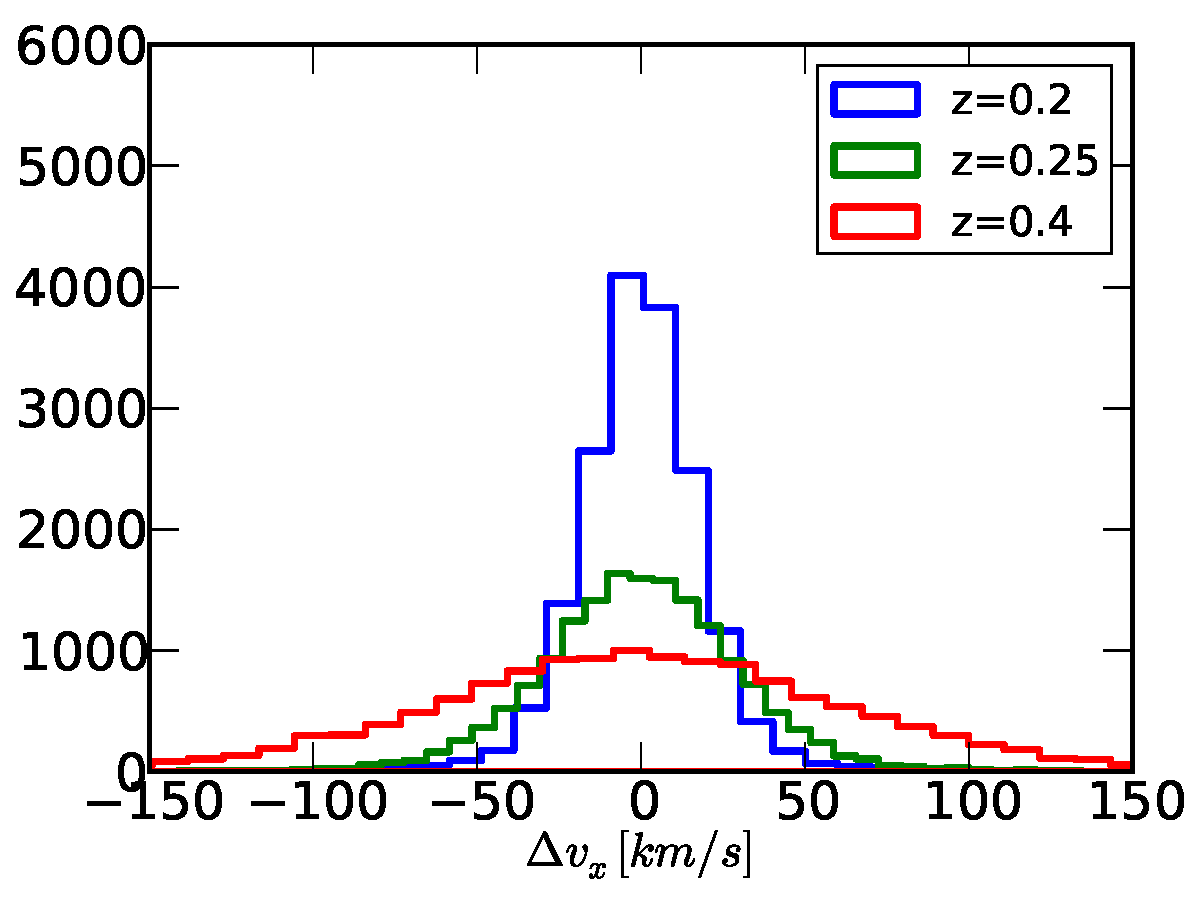
\includegraphics[width=0.5\columnwidth]{\lyxdot \lyxdot /Plots/hist_vx}\includegraphics[width=0.5\columnwidth]{\lyxdot \lyxdot /Plots/shifting_s_interp_z0\lyxdot 15}

\caption{\label{fig:lightcone_vel}\textcolor{black}{Left: Comparisons of the
$x$-component of velocities to the ones at $z=0.2$ before and after
linear interpolation. We estimate velocities at $z=0.2$ by linearly
interpolating velocities at $z=0.25$ and $z=0.15$. The blue line
shows the original scatter of the velocities between $z=0.25$ and
$z=0.2$, while the green line shows the scatter after linear interpolation.
Right: }The ratio of the power spectrum of the shifted halos to its
expected value in redshift space. We shift halos from $z=0.25$ to
$z=0.2$\textcolor{black}{{} and use original velocities at $z=0.25$
(blue line) and the linearly interpolated velocities (green line)
to define redshift space. The denominator is the redshift space cross
power spectra at $z=0.2$, which is an expected value after shifting.
As a reference, the result of shifting from $z=0.25$ to $z=0.2$
in real space is shown as a dashed line. }We recover the expected
power spectrum to better than $1\%$ out to $k=0.8h{\rm Mpc}^{-1}$\textcolor{black}{{}
by linearly interpolating velocities.}}
\end{figure}



\section{BOSS Mock Catalogs}

As a concrete implementation of the approach discussed above, we construct
catalogs designed to mimic the Baryon Oscillation Spectroscopic Survey
(hereafter, BOSS) galaxy samples. BOSS (\cite{2013AJ....145...10D}),
part of the SDSS-III project (\cite{2011AJ....142...72E}), is a spectroscopic
survey that has achieved percent level distance measurements using
the baryon acoustic oscillation technique (\cite{2014MNRAS.441...24A}).
The low redshift ($z<0.7$) distance measurements use two galaxy samples
: the LOWZ ($z<0.45$) and CMASS ($z<0.7$) samples (\cite{2014MNRAS.441...24A,2014MNRAS.440.2222T}).
We describe the construction of the CMASS sample below. The construction
of the LOWZ sample is analogous, and the same simulations (as different
time slices) can be used in its construction.

We choose a simulation volume large enough to build a full-sky mock
catalog. Since the CMASS sample extends to $z\sim0.7$, we choose
a simulation side of $4000h^{-1}{\rm Mpc}$, corresponding to a comoving
distance to $z\sim0.8$ from the center of the box. We start the simulations
at $z=200$ using Zel\textquoteright{}dovich initial conditions and
are run down to $z=0.15$ using the time-stepping procedure described
earlier in the paper. We store outputs every $\Delta z\sim0.05$ starting
at $z\sim0.75$; in addition, we store outputs uniformly spaced by
$\Delta z=0.2$ between $z=1$ and $z=2$ as well as at $z\sim2.5$,
$3$ and $4$. The close spacing at low redshift enables us to make
lightcones using the method described in the previous section. We
run a friends-of-friends halo finder on each of the outputs with a
linking length of $b=0.168$, keeping halos down to 40 particles,
or $10^{12.6}M_{\odot}$. By comparison, the characteristic halo mass
of the BOSS galaxies is $10^{13}M_{\odot}$, which we resolve with
100 particles. Each output store\textcolor{black}{s central positions,
mean velocities and halo masses , and $1\%$ of halo particles with
minimum of 5 particles per halo and $1\%$ of all particles randomly
sampled. }\textcolor{red}{We run the simulations with a range of cosmologies
centered at WMAP-7 (\cite{2011ApJS..192...18K}) and Planck (\cite{2015arXiv150201589P})
with varied $\sigma_{8}$, shown in Table \ref{tab:cosmology}. For
each model, we save one full simulation (meaning with very accurate
time stepping) out to $z=0$, and 5 realizations that have reduced
time steps out to $z=0.15$. In this section, we use four realizations
from the WMAP-7 cosmology with $\sigma_{8}=0.8$. For this case, one
realization was failed to save. }

\begin{table}
\begin{tabular}{|c|c|c|c|c|c|c|}
\hline 
 & WMAP-7 & WMAP-7 & WMAP-7 & Planck & Planck & Planck\tabularnewline
\hline 
\hline 
$\Omega_{m}$ & 0.265 & 0.265 & 0.265 & 0.315 & 0.315 & 0.315\tabularnewline
\hline 
$\Omega_{b}h^{2}$ & 0.02258 & 0.02258 & 0.02258 & 0.02202 & 0.02202 & 0.02202\tabularnewline
\hline 
$h$ & 0.71 & 0.71 & 0.71 & 0.673 & 0.673 & 0.673\tabularnewline
\hline 
$n_{s}$ & 0.963 & 0.963 & 0.963 & 0.96 & 0.96 & 0.96\tabularnewline
\hline 
$\sigma_{8}$ & 0.8 & 0.83 & 0.77 & 0.8 & 0.83 & 0.77\tabularnewline
\hline 
\end{tabular}

\caption{\label{tab:cosmology}\textcolor{red}{Cosmological parameters used
to run the simulation. For each model, we run one full simulation
(meaning with very accurate time stepping) out to $z=0$, and 5 realizations
that have reduced time steps out to $z=0.15$. }}
\end{table}


The BOSS angular geometry is split into two regions : one in the North
Galactic Cap and one in the South Galactic Cap (Figure~\ref{fig:boss-geom}).
Since we generate full-sky mocks, it is straightforward to embed two
full non-overlapping BOSS surveys in a single mock realization. We
cut out a first BOSS volume with $\vec{x}_{old}$ and then define
a new coordinate system $\vec{x}_{new}$ such that $\vec{x}_{new}=R\vec{x}_{old}$,
where $R$ is the Euler rotation matrix:
\[
R=\left(\begin{array}{ccc}
0.088 & 0.096 & 0.991\\
0.219 & -0.973 & 0.075\\
0.972 & 0.211 & -0.107
\end{array}\right).
\]


\begin{figure}[H]
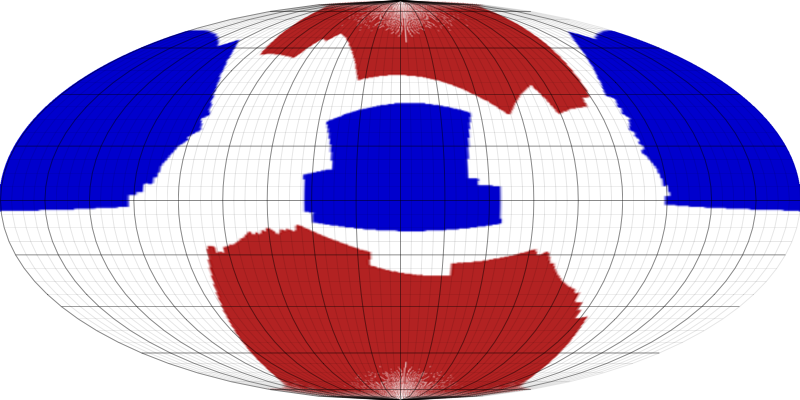
\includegraphics[width=0.5\columnwidth]{\lyxdot \lyxdot /Plots/boss_geom}

\caption{\label{fig:boss-geom}Fitting two non-overlapping BOSS volumes into
the same simulation box. The blue region is the BOSS survey footprint
in equatorial coordinates, while the red region is the same region
rotated using the rotation matrix given in the text.}
\end{figure}


To generate the galaxy mock catalogs, we first populate halos with
galaxies using a halo occupational distribution (HOD) approach. The
HOD functional form (based on a number of free parameters, 5 in our
case) provides probabilities for the number of central and satellite
galaxies based on the masses of halos that host those galaxies. A
halo hosts a central galaxy with probability $<N_{cen}(M)>$ and a
number of satellite galaxies given by a Poisson distribution with
mean $<N_{sat}(M)>$:

\begin{equation}
<N_{cen}(M)>=\frac{1}{2}{\rm erfc}\left[\frac{{\rm ln}(M_{cut}/M)}{\sqrt{2}\sigma}\right],\label{eq:Ncen}
\end{equation}
and 
\begin{equation}
<N_{sat}(M)>=N_{cen}(M)\left(\frac{M-\kappa M_{cut}}{M_{1}}\right)^{\alpha},\label{eq:Nsat}
\end{equation}
where $M_{cut}$, $M_{1}$, $\sigma$, $\kappa$, and $\alpha$ are
free parameters and $M$ is the halo mass. We assume that $N_{sat}(M)$
is zero when $M<\kappa M_{cut}$ and halos do not host satellite galaxies
without a central galaxy~\cite{2005ApJ...633..791Z}. The total number
of galaxies hosted by each halo is a sum of the number of central
and satellite galaxies. Equations~\ref{eq:Ncen} and \ref{eq:Nsat}
are not the only possible functional form for the HOD, and it is trivial
to change this. However, these forms are known to successfully reproduce
the clustering of the BOSS galaxies~\cite{2011ApJ...728..126W} and
are therefore a convenient choice.

After assigning a number of galaxies to each halo, we distribute those
galaxies within the halo. The central galaxy is always at the center
of the halo, while the distribution of satellite galaxies follow a
spherically symmetric NFW profile specified by: 
\begin{equation}
\rho(r)=\frac{4\rho_{s}}{\frac{cr}{R_{{\rm vir}}}(1+\frac{cr}{R_{{\rm vir}}})^{2}},
\end{equation}
where $\rho_{s}$ is the density at the char\textcolor{black}{acteristic
scale $r_{s}=R_{{\rm vir}}/c$ , $R_{{\rm vir}}$ is the virial radius
for the halo and $c$ is the concentration parameter. $R_{{\rm vir}}$
is the virial radius of the halo}.\textcolor{black}{{} We use a cosmic
emulator \cite{2013ApJ...768..123K} to generate a table of concentration-mass
relation for halos at each redshift with the given cosmology.}

The velocity of the central galaxy is equal to the host halo velocity.
We assume that satellite galaxies are randomly moving inside the host
halos. Therefore, the velocities of the satellite galaxies are the
sum of their host halo velocity and a random virial component. For
this random component, we draw a Gaussian distribution with zero mean
and variance given by:

\begin{equation}
<v_{x}^{2}>=<v_{y}^{2}>=<v_{z}^{2}>=\frac{1}{3}\frac{GM}{R_{vir}}.\label{eq:variance}
\end{equation}


Following the above procedures, we generate two galaxy mocks from
the simulation at $z=0.55$ and from the lightcone sample described
in Section 4. Using the simulation at $z=0.55$ is the way to generate
galaxy mocks described in Ref. \cite{2013MNRAS.428.1036M,2014arXiv1401.4171M}
and used in \cite{2014MNRAS.441...24A}, The reason we also generate
a galaxy mock from the lightcone sample is to explore whether those
two galaxy mocks exhibit any differences or not.\textcolor{black}{{}
We use the following HOD parameters, $M_{cut}=12.9$, $M_{1}=14.0$,
$\alpha=1.013$, $\kappa=1.0$, $\sigma=0.85$, to populate the halos
with galaxies. Note that the goal here is not to completely fit to
the observed DR11 correlation functions, but to show that our simulations
have capability to compute correlation functions for BOSS.}

\textcolor{black}{Once generating the galaxy mocks, the next step
is matching the number density $n(z)$ to the redshift selection function
of Ref. \cite{2013arXiv1303.4666A}. For each redshift bin, we randomly
subsample galaxies. Figure \ref{fig:nz_gal} shows redshift distributions
of galaxies before and after subsampling for BOSS CMASS North Galactic
Cap, which correspond to dashed and solid lines respectively. The
blue solid line is the redshift distribution of galaxies for BOSS,
while the green and red line represents $n(z)$ from the mock at $z=0.55$
and the lightcone sample. }

\textcolor{black}{After matching the redshift distribution of galaxies,
we finally compute correlation functions for those galaxy mocks. In
Figure \ref{fig:xis}, we compare those correlation functions to the
one from DR11. The left panel shows the monopole terms of the correlation
functions, and the right panel is the quadrupole terms. We do not
see siginificant differences between the galaxy mocks from the simulation
at $z=0.55$ and the lightcone sample for both monopole and quadrupole
terms. For the monopole terms, the mocks agree relatively well with
the one from DR11 on $r\in[40h^{-1}{\rm Mpc},80h^{-1}{\rm Mpc}]$.
Note that we do not try to fit to the acoustic peak hear, because
the cosmologies for our simulation and DR11 are different. On the
other hand, we fail to fit the quedrupole terms to the observed quadrupole
term from DR11 by overestimating the power, which also happens in
Ref. \cite{2014MNRAS.437.2594W}. }

\begin{figure}
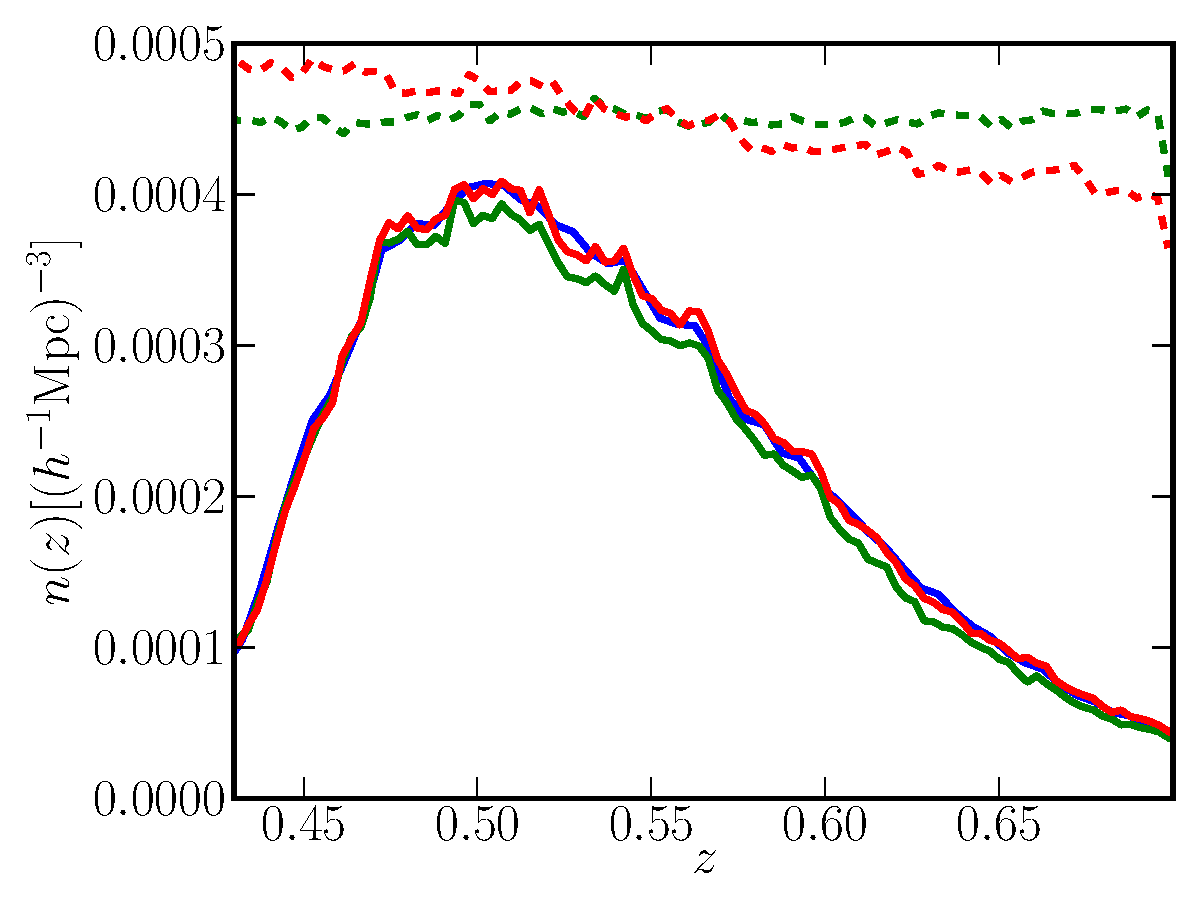
\includegraphics[width=0.5\columnwidth]{\lyxdot \lyxdot /Plots/nz_dr11_N}

\caption{\label{fig:nz_gal}\textcolor{red}{Normalized redshift distribution
of galaxies from DR11 (North) in Ref.~\cite{2013arXiv1303.4666A}
(blue solid line), and a comparison of galaxy number densities before
fitting to DR11 redshift selection function (dashed lines) and after
(solid lines). The green and red lines are from the mocks at $z=0.55$
and the lightcone output respectively. The HOD parameters used to
generate the mock catalogs can be found in text.}}
\end{figure}


\begin{figure}
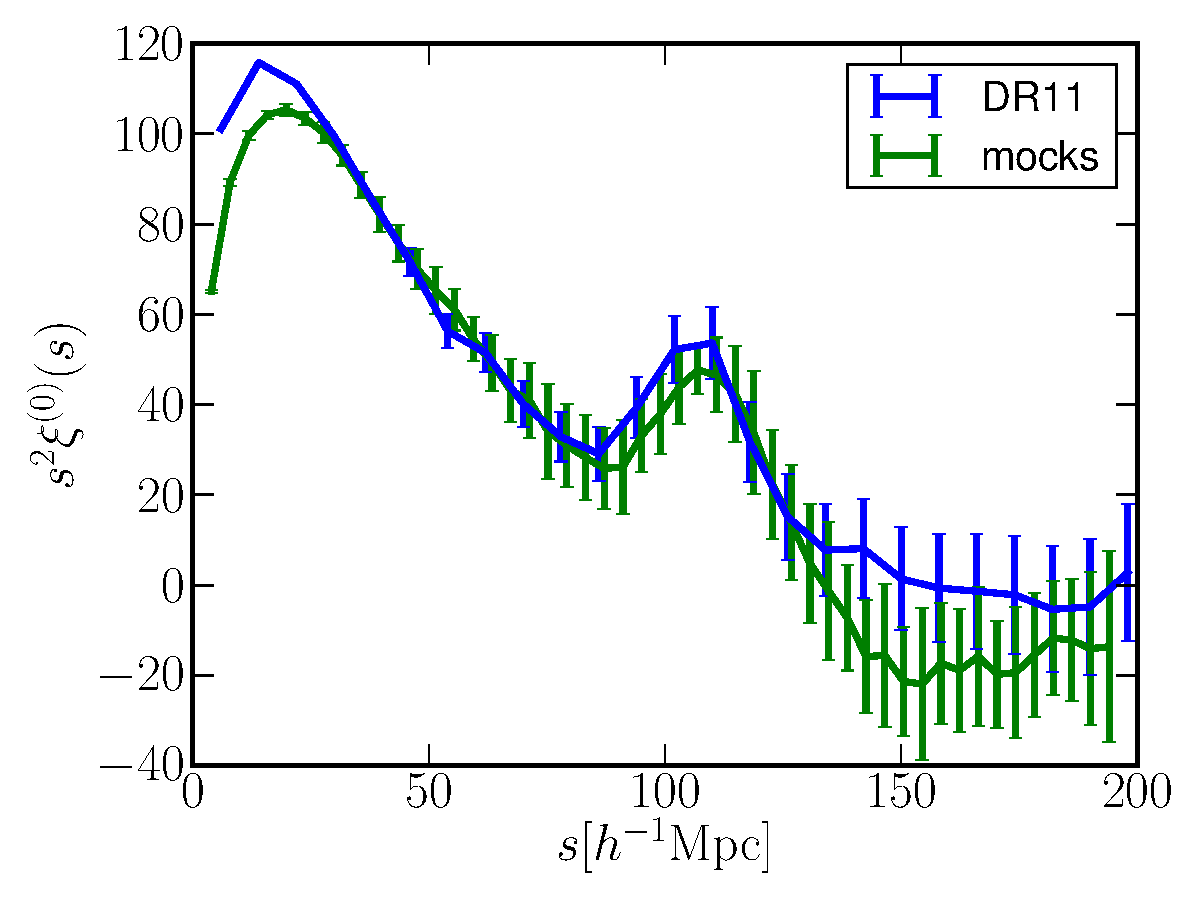
\includegraphics[width=0.5\columnwidth]{\lyxdot \lyxdot /Plots/xi0_obs}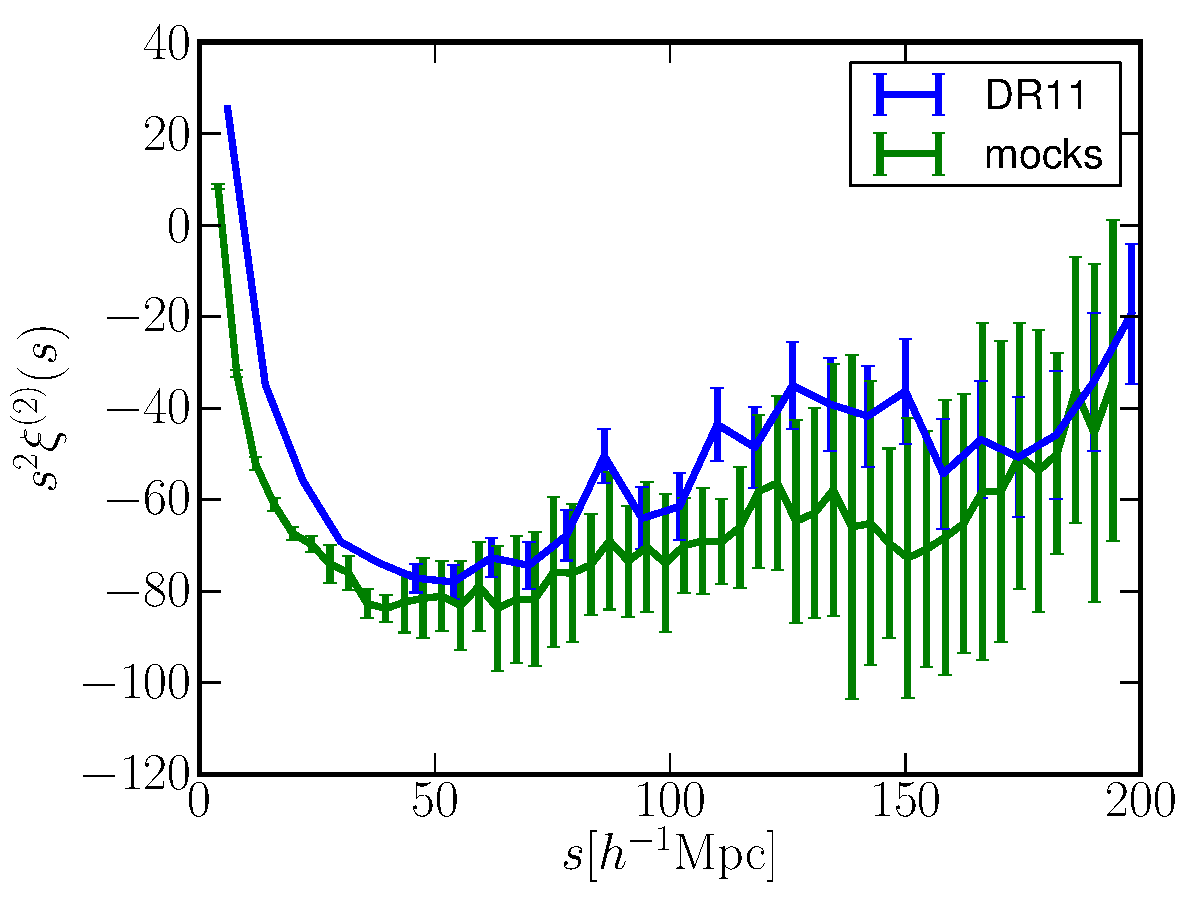
\includegraphics[width=0.5\columnwidth]{\lyxdot \lyxdot /Plots/xi2_obs}

\caption{\label{fig:xis}Correlation function monopoles $\xi^{(0)}(s)$ (left)
and quadrupoles $\xi^{(2)}(s)$ (right) of the mocks (green and red)
and DR11 in Ref.~\cite{2013MNRAS.428.1036M} (blue) at $z=0.55$.
The HOD parameters used to generate the mock catalogs can be found
in text.}
\end{figure}


One of the other applications of those mocks is to use the mock correlation
functions as a template function, which we discuss in detail in Section
5.1, to fit to an observed correlation function. As a demonstration,
we fit our mock correlation functions to the one from DR11. We use
the mock correlation function as a template shown in Eq. \ref{eq:model1}
and measure the value of $\alpha$, which is the scale dilation parameter
measuring the relative distance scales between observations and the
fiducial model. This parameter $\alpha$ is related to the ratio:
\begin{equation}
\alpha\equiv\left(\frac{D_{{\rm V}}(z)}{r_{{\rm d}}}\right)\left(\frac{r_{{\rm d,fid}}}{D_{{\rm V}}^{{\rm fid}}(z)}\right),\label{eq:alpha_ratio}
\end{equation}
where $r_{{\rm d}}$ is the projection of the sound horizon at the
drag epoch and $D_{{\rm V}}\equiv\left[cz(1+z)^{2}D_{{\rm A}}(z)^{2}H^{-1}(z)\right]^{1/3}$
where $D_{{\rm A}}$ is the angular diameter distance and $H(z)$
is the Hubble parameter. The ratio $\left(\frac{r_{{\rm d,fid}}}{D_{{\rm V}}^{{\rm fid}}(z)}\right)$
for our simulations is 13.44 at $z=0.57$, while the ratio $\left(\frac{D_{{\rm V}}(z)}{r_{{\rm d}}}\right)$
from DR11 is $13.91\pm0.13$. So, the estimated value for $\alpha$
is $1.025\pm0.010$.

Figure \ref{fig:alpha_fit} shows the $\chi^{2}$ values as a function
of the parameter $\alpha$ in the left panel and compares the monopole
correlation function from DR11 and the fitted function in the right
panel. We obtain the value of $1.033\pm0.012$, which is within $1\sigma$
from the estimated value for $\alpha$. This demonstrates that our
simulations can be used as a template function to measure the shift
in the acoustic peak.

\begin{figure}[H]
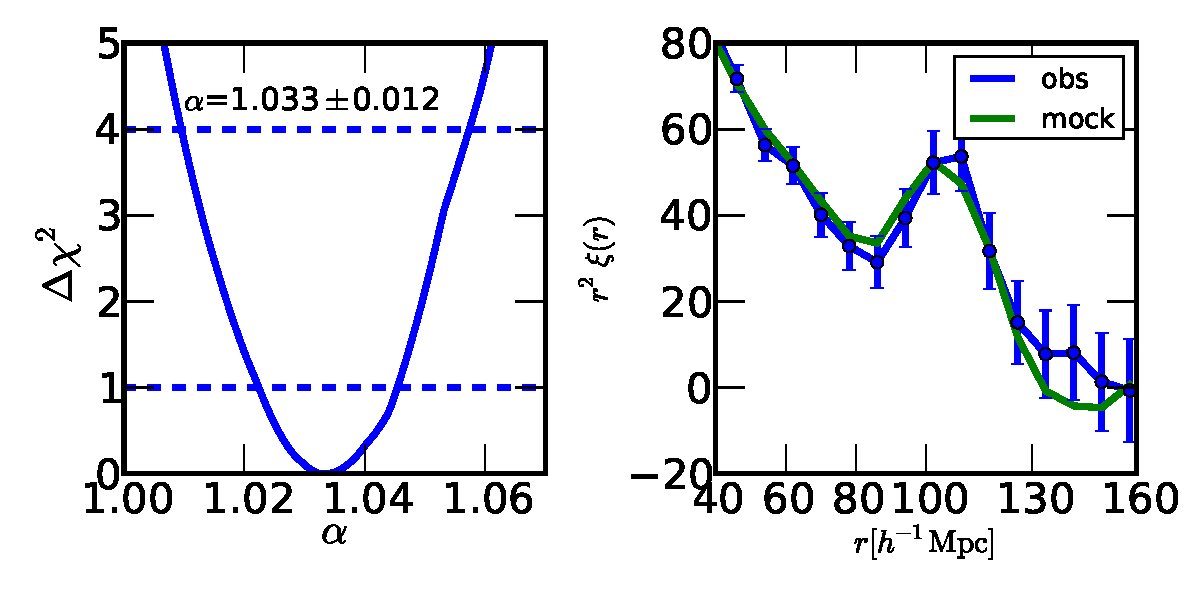
\includegraphics[width=1\columnwidth]{\lyxdot \lyxdot /Plots/xi_lightcone}

\caption{\label{fig:alpha_fit}Left: Plot of $\Delta\chi^{2}$ vs. $\alpha$
for the data from DR11. The dashed lines (from top to bottom) correspond
to $2\sigma$ and $1\sigma$ for the value of $\alpha$. The best
fit value of $\alpha$ is $1.033\pm0.012$. Right: The monopole correlation
functions of the data from DR11 (blue line) and of the lightcone galaxy
mock fitted with $\alpha=1.033$.}
\end{figure}



\subsection{Testing the shift of the BAO peaks}

As a second application of this suite of simulations, we explore how
the baryon acoustic oscillation (hereafter BAO) changes as a function
of changing galaxy bias. These shifts, predicted by basic perturbative
arguments (e.g.. \cite{2008PhRvD..77b3533C,2009PhRvD..80f3508P,2012PhRvD..85j3523S}),
must be calibrated at the sub percent level for future BAO experiments
as a function of the underlying cosmology and galaxy type. Measuring
these shifts requires large simulation volumes to robustly measure
them from under the statistical error. The approximations we describe
in this paper allow such large volumes to be run, without sacrificing
the gross details (positions, masses, velocities) of the halos themselves
(which, in turn, allow one to construct mock galaxy populations).
Note that our goal here is to demonstrate the statistical power of
these simulations, deferring an exhaustive study to later work.

In order to construct samples of different galaxy biases, we construct
realizations of HODs with the same parameters as in Sec 5.1, except
for $M_{cut}$ which we vary from 12.5 to 14.1 in steps of 0.2. The
resulting nine HODs span a range of biases from 1.5 to 3.5. In order
to estimate the covariance matrix for galaxy correlation functions,
we subdivide each of our $4\times(4h^{-1}{\rm Gpc})^{3}$ volumes
into $4\times64=256$ subvolumes. For simplicity, we analyze each
of these subvolumes individually, except for the Mcut=13.9 and 14.1
samples where we analyze groups of 4 sub volumes to reduce the noise
in the measurements. %
\footnote{In these cases, we scale the covariance matrix by a factor of 1/4.%
} We focus here on real-space measurements. 

We measure the BAO scale using the methodology in Ref. \cite{2013arXiv1303.4666A}.
Specifically, we describe the observed correlation function by $\xi_{{\rm fit}}$:
\begin{equation}
\xi_{{\rm fit}}(r)=B\xi_{t}(\alpha r)+A_{0}+A_{1}/r+A_{2}/r^{2},\label{eq:model1}
\end{equation}
where $\xi_{t}$ is a template correlation function, $B$ is the galaxy
bias squared and $A_{0,1,2}$ represent nuisance parameters to account
for shot noise, nonlinear evolution of the matter density field and
the mapping from matter to galaxies (\textcolor{red}{NEED TO FIND
A BETTER PHRASE FOR THE LAST}; the galaxy distribution as a biased
tracer of matter). The template correlation function $\xi_{t}(r)$
is given by Fourier transforming $P_{t}(k)$:
\begin{equation}
P_{t}(r)=(P_{{\rm lin}}(k)-P_{nw}(k))e^{-\frac{k^{2}\Sigma^{2}}{2}}+P_{nw}(k),
\end{equation}
where $ $$P_{{\rm lin}}(k)$ is the linear power spectrum and $P_{nw}(k)$
is the no-wiggle power spectrum described in Ref. \cite{1998ApJ...496..605E},
and $\Sigma$ is a nonlinear para\textcolor{black}{meter which accounts
for broadening the BAO peak due to non-linear evolution. We set $\Sigma=5h^{-1}{\rm Mpc}$.
We determine the parameters by minimizing $\chi^{2}=(\xi_{{\rm HOD}}-\xi_{{\rm fit}})^{{\rm T}}C^{-1}(\xi_{{\rm HOD}}-\xi_{{\rm fit}})$
where $C^{-1}$ is the inverse covariance matrix and $\xi_{{\rm HOD}}$
is a correlation function which $\xi_{{\rm fit}}$ is fitted to. W}e
consider the measured correlation function from $60h^{-1}{\rm Mpc}$
to $160h^{-1}{\rm Mpc}$ in bins of $4h^{-1}{\rm Mpc}$ for a total
of 25 data points. Since all parameters except $\alpha$ are linear,
we perform the minimization on a grid of $\alpha$ values, computing
the minimum value of the other parameters directly. The parameter
$\alpha$ measures the shift of the BAO peak from its original position
predicted by the linear perturbation theory. Note that $\alpha=1$
implies that there is no shift of the BAO peak.

The left panel of Figure \ref{fig:demo} compares the correlation
function computed from one of the full boxes with $M_{cut}=12.9$
(which corresponds to the galaxy bias of 1.81) and the model correlation
function described in Eq. \ref{eq:model1} with the best-fit parameters.
The best fit value of $\alpha$ for this mock is 1.003. Note that
the error bars shown in the left panel of Figure \ref{fig:demo} are
computed from the covariance matrix. The right panel of Figure \ref{fig:demo}
shows the distribution of $\alpha-1$ for the case of $M_{cut}=12.9$
for the 256 samples. The mean value of $\alpha-1$ is $0.0068\pm0.0012$.

\begin{figure}[H]
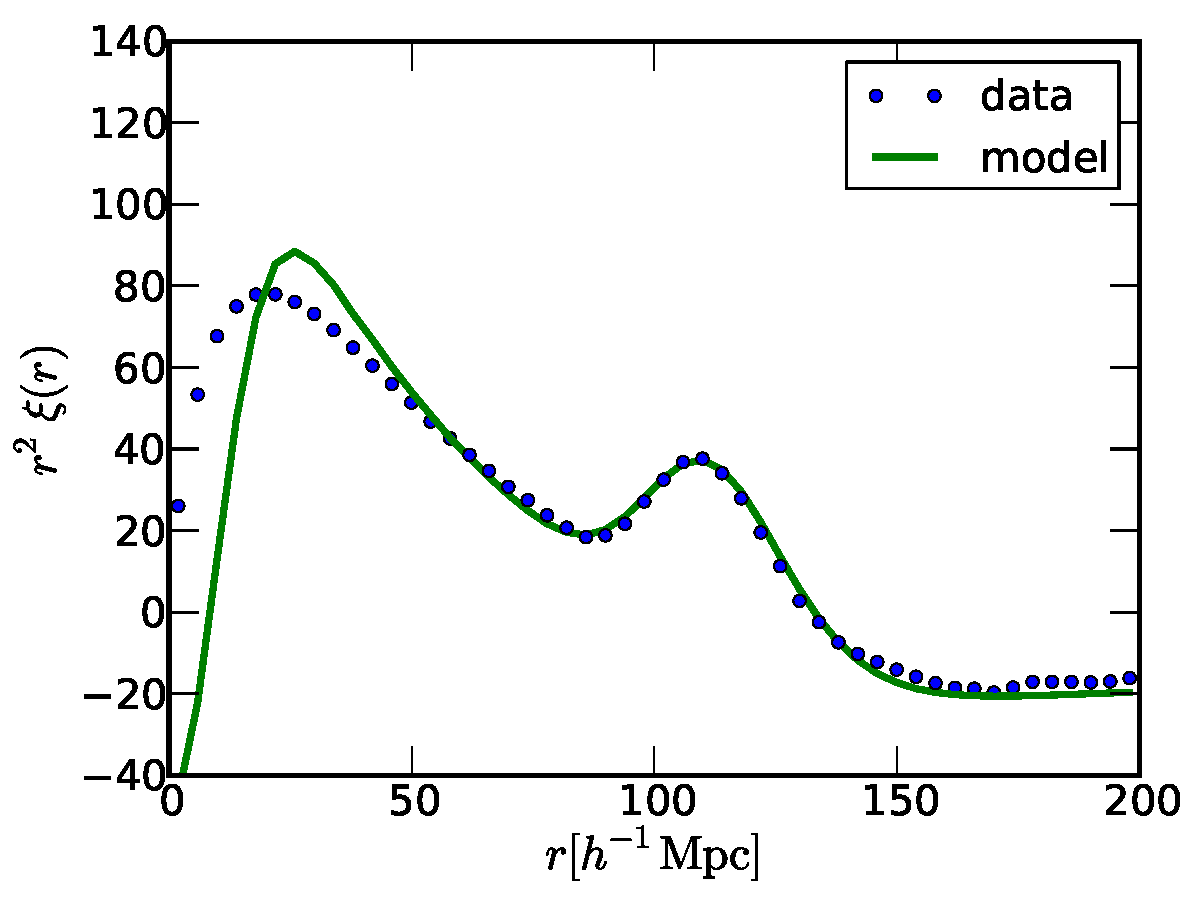
\includegraphics[width=0.5\columnwidth]{\lyxdot \lyxdot /Plots/xi_hod3}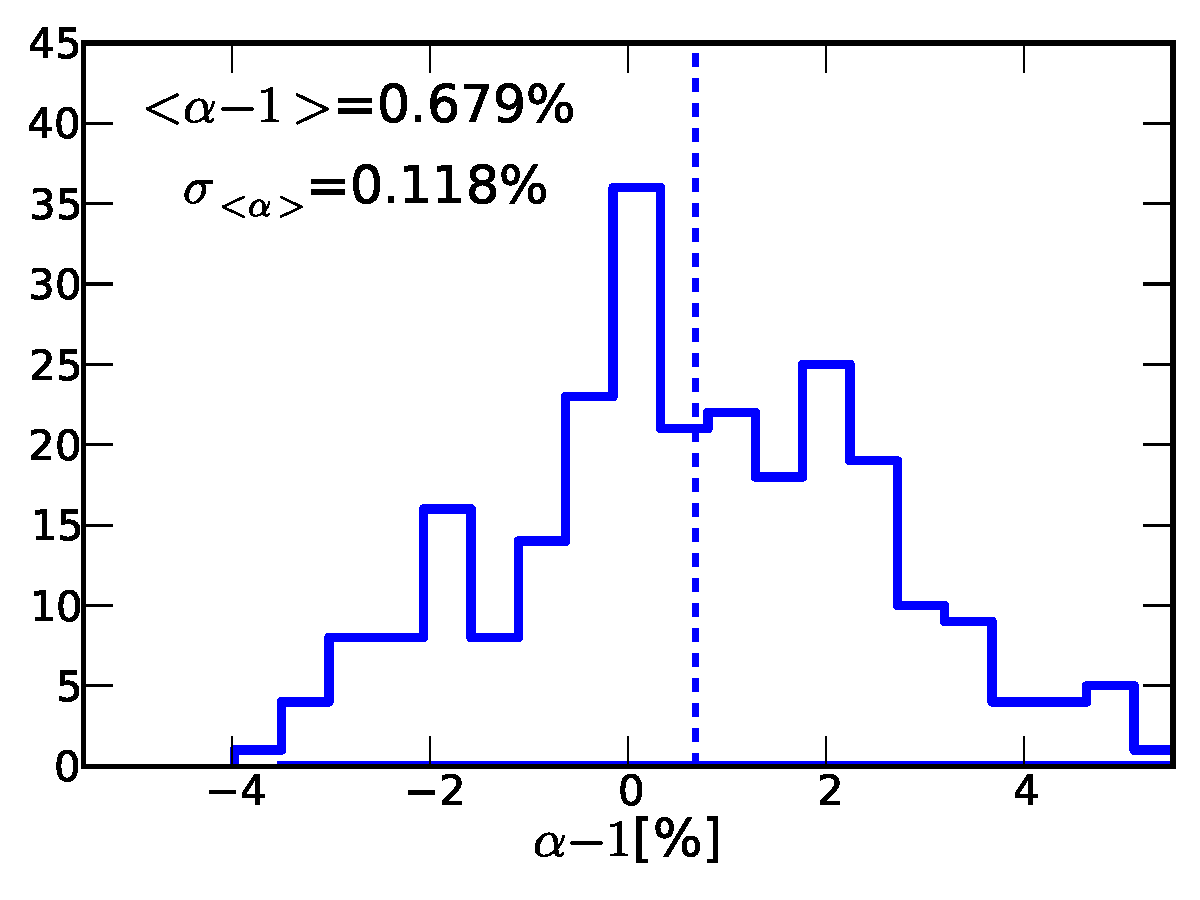
\includegraphics[width=0.5\columnwidth]{\lyxdot \lyxdot /Plots/alpha_hist_hod3}

\caption{\label{fig:demo}Left: The correlation function $\xi_{{\rm HOD}}(r)$
computed from the full HOD galaxy mock (labeled as ``data'') with
$M_{cut}=12.9$ (which corresponds to the bias value of 1.81) and
the template correlation function with the best-fit parameters (labeled
as ``model''). The best fit value of $\alpha$ for this mock is
1.003. The error bars are computed from the covariance matrix. Right:
Distribution of the values $\alpha-1$ for the case of $M_{cut}=12.9$.
The dashed line corresponds to the mean value of $\alpha-1$, which
is 0.006.}
\end{figure}


Figure \ref{fig:alpha} shows the measured shifts in the BAO scale
as a function of galaxy bias, for the nine HODs described above. We
detect the shift in the BAO scale at high significance ($\sim6\sigma$
for most samples) but do not detect a strong variation with the galaxy
bias. Indeed, the shift is consistent with being constant for biases
> 3.0 and only increases for extremely large biases. These results
agree with the trends in Ref. \cite{2011ApJ...734...94M}, although
note that the absolute values of the shifts differ since Ref. \cite{2011ApJ...734...94M}
consider samples at $z=1$, while the results here are at $z=0.15$.
We also observe that our results are roughly consistent with what
one expects from perturbation theory (\cite{2008PhRvD..77b3533C,2009PhRvD..80f3508P,2012PhRvD..85j3523S}),
although we find a weaker mass dependence than what was predicted
by Ref. \cite{2009PhRvD..80f3508P}.

This work can be extended by using reconstruction on the sample to
verify that it does indeed reduce these biases both in real-space
and in redshift-space, comparing to the perturbation theory \textcolor{black}{results},
testing redshift evolution and cosmology dependence in the shift of
the peak.

\begin{figure}[H]
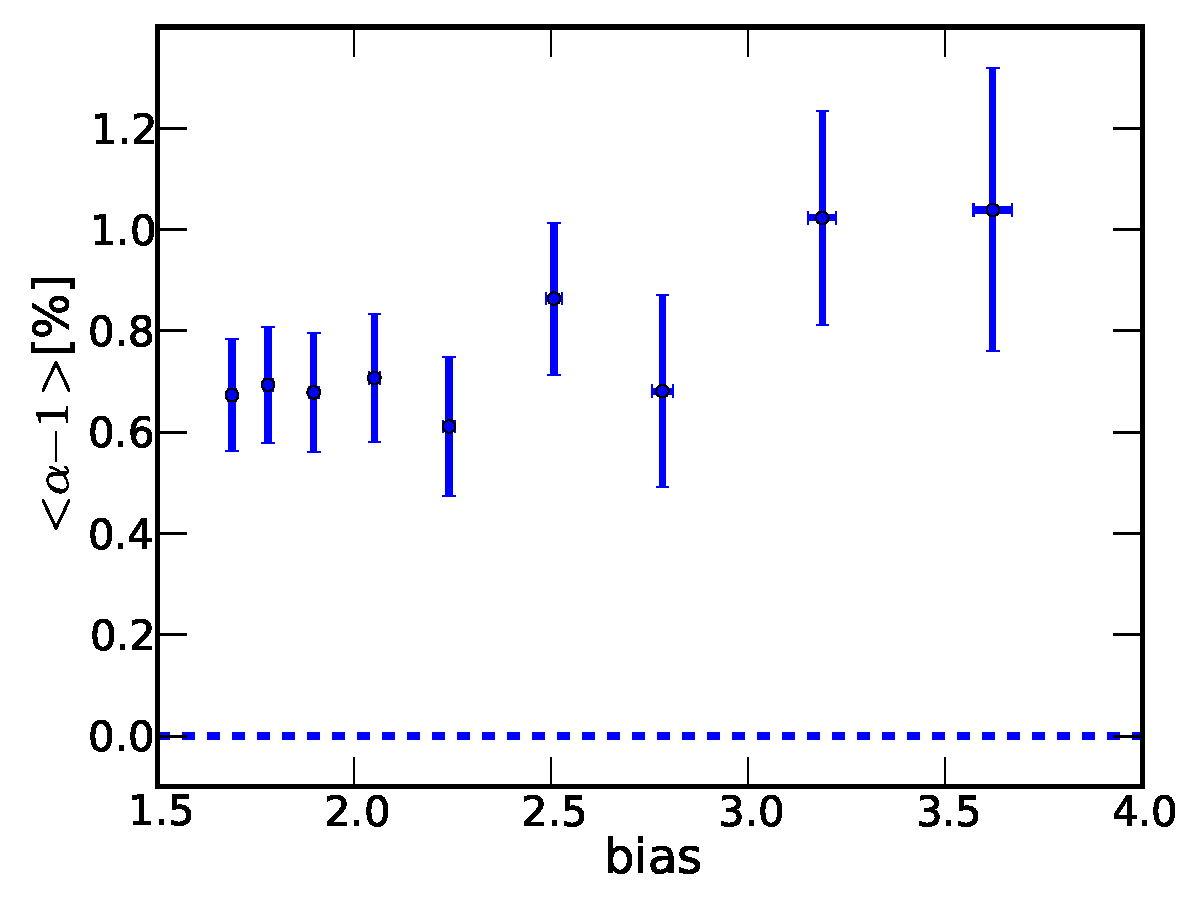
\includegraphics[width=0.5\columnwidth]{\lyxdot \lyxdot /Plots/alpha_bias}

\caption{\label{fig:alpha}The shift in the BAO scale as a function of galaxy
bias. Note that $\alpha-1$ implies no shift in the BAO scale. We
detect a significant shift ($\sim6\sigma$ for most cases) for all
the samples we consider. The shift is consistent with being constant
for biases > 3.0 and only increases for extremely large biases. These
results agree with the trends in Ref. \cite{2011ApJ...734...94M}.
The third point from left uses the HOD parameter of $M_{cut}=12.9$,
which are the same samples used in Figure \ref{fig:demo}. }
\end{figure}



\section{Discussion}

Precision required for current and future galaxy spectroscopic surveys
to test the expansion and structure formation histories of the Universe
requires an accurate understanding of systematic effects. In this
paper we have presented a quantitative study of the impact of time
step sizes on the halo and matter density fields. Our code has two
adjustable time stepping parameters - a global time step and a number
of sub-cycles (responsible for a particle-particle interactions) to
track that particle trajectories on small scales. We consider cases
where we increase the length of each time step by factors of 1.5 and
3 respectively, as well as reducing the number of sub-cycles. Our
fiducial choice is to use using 300 global time steps corresponding
to $\Delta a(z)=0.003$ and 2 sub-cycles (increasing the length of
the global time step by a factor of 1.5 and that of the sub-cycles
by a factor of 2.5), resulting in a reduction of the simulation run
time by 4 times less. We keep the mass resolution constant; the results
here are based on a particle mass of $6.86\times10^{10}h{\rm M_{\odot}}$.We
summarize the key results below:

(a) The halo masses tend to be underestimated in these cases, as one
might expect because reducing the number of time steps produces halos
with less substructure and a more diffuse distribution of mass. However,
this trend may be calibrated with smaller simulations and corrected,
recovering the halo masses to 98\%. The halo mass function is correctly
recovered fully for masses above $10^{12.7}h^{-1}{\rm M_{\odot}}$
corresponding to 100 particles. Note that we run the halo finder with
identical parameters as in the full resolution runs. It may however
be possible to get similar results by changing the parameters of the
halo finder, as was done in \cite{2013MNRAS.428.1036M}.

(b) \textcolor{black}{The halo positions and velocities are recovered
with a scatter of $0.08[h^{-1}{\rm Mpc}]$ and $12.8[{\rm km/s}]$
respectively for the simulation of our fiducial choice. }

(c) The clustering of these halos is correctly recovered to better
than 1\% on scales below $k<1[h{\rm Mpc^{-1}]}$ in real-space and
$k<0.5[h{\rm Mpc^{-1}}]$.

(d) We find that the number of sub-cycles makes almost no difference
to any of our final results.

\textcolor{black}{We also consider the redshift sampling required
to construct light cone outputs. We first compare the distances for
the halos at different redshifts before and after shifting their positions
from one redshift to the another. Moving halos over a $\Delta z=0.1$
interval correctly reduces the standard deviation of those distances
from $0.25[h^{-1}{\rm Mpc}]$ to}\textcolor{red}{{} }\textcolor{black}{$0.09[h^{-1}{\rm Mpc}]$.
Moreover, the power spectra are correctly recovered to better than
1\% for $k<1h{\rm Mpc}^{-1}$ for $\Delta z<0.25$. }\textcolor{red}{This
worsens in redshift space to 2\% up to $k<0.2h{\rm Mpc}^{-1}$ by
assuming that the change in velocity across the simulations is negligible
and using the original velocity to compute redshift space. The agreement
is, however, improved to 1\% for $k<0.8h{\rm Mpc}^{-1}$ by using
the velocity linearly interpolated between the snapshots and the true
redshift. }\textcolor{black}{Our fiducial choice to construct light
cone outputs is $\Delta z=0.05$.}

This work is a natural extension of the approaches described in \cite{2014MNRAS.439L..21K,2014MNRAS.437.2594W,2014arXiv1409.1124C,2013MNRAS.428.1036M,2014arXiv1401.4171M}.
The primary goal for those papers was to generate the large numbers
of simulations required for estimating covariance matrices. We quantify,
in detail, the impact of size of the time step on large scale observables;
our suite of simulations are better designed for testing for systematic
errors in theory and analysis techniques. As a proof of principle,
we present a set of eight full BOSS (both North and South Galactic
caps simultaneously) simulations. The time savings presented in this
paper allowed to extend this to 50 simulations, across a range of
cosmolog\textcolor{black}{ies centered at WMAP-7 (\cite{2011ApJS..192...18K})
and Planck (\cite{2015arXiv150201589P}) with varied $\sigma_{8}$.
}These results from these will be presented in future publications.


\section*{Acknowledgement}

TS and NP are supported by a DOE Early Career Grant. This work was
supported in part by the facilities and staff of the Yale University
Faculty of Arts and Sciences High Performance Computing Center, and
by resources at the National Energy Research Scientific Computing
Center. TS would like to thank Andrew Szymkowiak for useful discussions.
This research used resources of the National Energy Research Scientific
Computing Center, a DOE Office of Science User Facility supported
by the Office of Science of the U.S. Department of Energy under Contract
No. DE-AC02-05CH11231. Argonne National Laboratory's work was supported
under U.S. Department of Energy contract DE-AC02-06CH11357.

\bibliographystyle{JHEP}
\bibliography{bigsims}

\end{document}
